\documentclass[mathserif]{beamer}

\setbeamertemplate{frametitle}[default][center]%Centers the frame title.
\setbeamertemplate{navigation symbols}{}%Removes navigation symbols.
\setbeamertemplate{footline}{\raisebox{5pt}{\makebox[\paperwidth]{\hfill\makebox[10pt]{\scriptsize\insertframenumber}}}}
\setbeamertemplate{caption}[numbered]

\usepackage{amssymb,amsfonts,amsmath,latexsym,amsthm}
%\usepackage[usenames,dvipsnames]{color}
%\usepackage[]{graphicx}
%\usepackage[space]{grffile}
\usepackage{mathrsfs}   % fancy math font
% \usepackage[font=small,skip=0pt]{caption}
\usepackage[skip=0pt]{caption}
\usepackage{subcaption}
\usepackage{verbatim}
\usepackage{url}
\usepackage{bm}
\usepackage{dsfont}
\usepackage{extarrows}
\usepackage{multirow}
%\newcommand{\tth}   {\mbox{$\theta$}}
\newcommand{\thh}   {\mbox{$\theta$}}
\newcommand{\su}   {\mbox{$\sigma^2$}}
\newcommand{\so}   {\mbox{$\sigma_0^2$}}
\newcommand{\ko}   {\mbox{$\kappa_0$}}
\newcommand{\no}   {\mbox{$\nu_0$}}
\newcommand{\mo}   {\mbox{$\mu_0$}}
\newcommand{\ti}   {\mbox{$\tilde{x}$}}
\newcommand{\la}   {\mbox{$\lambda$}}
\newcommand{\bx}   {\mbox{$\bm{x}$}}
\newcommand{\bZ}   {\mbox{$\bm{Z}$}}
\newcommand{\bX}   {\mbox{$\bm{X}$}}
\newcommand{\bY}   {\mbox{$\bm{Y}$}}
\newcommand{\bA}   {\mbox{$\bm{A}$}}
\newcommand{\ba}   {\mbox{$\bm{a}$}}
\newcommand{\bb}   {\mbox{$\bm{b}$}}
\newcommand{\bt}   {\mbox{$\bm{t}$}}
\newcommand{\bz}   {\mbox{$\bm{z}$}}
\newcommand{\bw}   {\mbox{$\bm{w}$}}
\newcommand{\bbeta}   {\mbox{$\bm{\beta}$}}

\newcommand{\be}   {\mbox{$\bm{e}$}}
\newcommand{\bu}   {\mbox{$\bm{u}$}}
\newcommand{\bv}   {\mbox{$\bm{v}$}}
\newcommand{\sig}   {\mbox{$\Sigma$}}
\newcommand{\sigx}   {\mbox{$\Sigma_{XX}$}}
\newcommand{\sigxy}   {\mbox{$\Sigma_{XY}$}}
\newcommand{\tr}   {\mbox{$\text{tr}$}}
\newcommand{\ddet}   {\mbox{$\text{det}$}}
\newcommand\independent{\protect\mathpalette{\protect\independenT}{\perp}}
\def\independenT#1#2{\mathrel{\rlap{$#1#2$}\mkern2mu{#1#2}}}

\newcommand{\Expect}[1]{\ensuremath{\mathbf{E}\left[ #1 \right]}}
%\newcommand{\Var}[1]{\ensuremath{\mathrm{Var}\left[ #1 \right]}}
%\newcommand{\Cov}[1]{\ensuremath{\mathrm{Cov}\left[ #1 \right]}}
\newcommand{\MSE}{\ensuremath{\mathrm{MSE}}}
\newcommand{\RSS}{\ensuremath{\mathrm{RSS}}}
\newcommand{\Prob}[1]{\ensuremath{\mathrm{Pr}\left( #1 \right)}}
\newcommand{\ProbEst}[1]{\ensuremath{\widehat{\mathrm{Pr}}\left( #1 \right)}}
\DeclareMathOperator*{\argmin}{argmin} % thanks, wikipedia!
\DeclareMathOperator*{\argmax}{argmax} % thanks, wikipedia!
\DeclareMathOperator*{\sgn}{sgn} % thanks, wikipedia!

\newcommand{\lam}{\lambda}
\newcommand{\bmu}{\bm{\mu}}
%\newcommand{\bx}{\ensuremath{\mathbf{X}}}
\newcommand{\X}{\ensuremath{\mathbf{X}}}
\newcommand{\w}{\ensuremath{\mathbf{w}}}
\newcommand{\h}{\ensuremath{\mathbf{h}}}
\newcommand{\V}{\ensuremath{\mathbf{V}}}
%\newcommand{\tr}{\operatorname{tr}}

%\newcommand{\bx}{\ensuremath{\mathbf{X}}}
%\newcommand{\X}{\ensuremath{\mathbf{x}}}
%\newcommand{\w}{\ensuremath{\mathbf{w}}}
%\newcommand{\h}{\ensuremath{\mathbf{h}}}
%\newcommand{\V}{\ensuremath{\mathbf{v}}}
%\newcommand{\Cov}{\text{Cov}}
%\newcommand{\Var}{\text{Var}}

\DeclareMathOperator{\var}{Var}
\DeclareMathOperator{\cov}{Cov}
\newcommand{\Var}[1]{\ensuremath{\mathrm{Var}\left[ #1 \right]}}
\newcommand{\Cov}[1]{\ensuremath{\mathrm{Cov}\left[ #1 \right]}}


\newcommand{\indep}{\rotatebox{90}{\ensuremath{\models}}}
\newcommand{\notindep}{\not\hspace{-.05in}\indep}







\usepackage{float,bm}
\floatstyle{boxed}
\newfloat{code}{tp}{code}
\floatname{code}{Code Example}
%\newcommand{\tth}   {\mbox{$\theta$}}
\newcommand{\thh}   {\mbox{$\theta$}}
\newcommand{\su}   {\mbox{$\sigma^2$}}
\newcommand{\so}   {\mbox{$\sigma_0^2$}}
\newcommand{\ko}   {\mbox{$\kappa_0$}}
\newcommand{\no}   {\mbox{$\nu_0$}}
\newcommand{\mo}   {\mbox{$\mu_0$}}
\newcommand{\ti}   {\mbox{$\tilde{x}$}}
\newcommand{\la}   {\mbox{$\lambda$}}
\newcommand{\bx}   {\mbox{$\bm{x}$}}
\newcommand{\bZ}   {\mbox{$\bm{Z}$}}
\newcommand{\bX}   {\mbox{$\bm{X}$}}
\newcommand{\bY}   {\mbox{$\bm{Y}$}}
\newcommand{\bA}   {\mbox{$\bm{A}$}}
\newcommand{\ba}   {\mbox{$\bm{a}$}}
\newcommand{\bb}   {\mbox{$\bm{b}$}}
\newcommand{\bt}   {\mbox{$\bm{t}$}}
\newcommand{\bz}   {\mbox{$\bm{z}$}}
\newcommand{\bw}   {\mbox{$\bm{w}$}}
\newcommand{\bbeta}   {\mbox{$\bm{\beta}$}}

\newcommand{\be}   {\mbox{$\bm{e}$}}
\newcommand{\bu}   {\mbox{$\bm{u}$}}
\newcommand{\bv}   {\mbox{$\bm{v}$}}
\newcommand{\sig}   {\mbox{$\Sigma$}}
\newcommand{\sigx}   {\mbox{$\Sigma_{XX}$}}
\newcommand{\sigxy}   {\mbox{$\Sigma_{XY}$}}
\newcommand{\tr}   {\mbox{$\text{tr}$}}
\newcommand{\ddet}   {\mbox{$\text{det}$}}
\newcommand\independent{\protect\mathpalette{\protect\independenT}{\perp}}
\def\independenT#1#2{\mathrel{\rlap{$#1#2$}\mkern2mu{#1#2}}}

\newcommand{\Expect}[1]{\ensuremath{\mathbf{E}\left[ #1 \right]}}
%\newcommand{\Var}[1]{\ensuremath{\mathrm{Var}\left[ #1 \right]}}
%\newcommand{\Cov}[1]{\ensuremath{\mathrm{Cov}\left[ #1 \right]}}
\newcommand{\MSE}{\ensuremath{\mathrm{MSE}}}
\newcommand{\RSS}{\ensuremath{\mathrm{RSS}}}
\newcommand{\Prob}[1]{\ensuremath{\mathrm{Pr}\left( #1 \right)}}
\newcommand{\ProbEst}[1]{\ensuremath{\widehat{\mathrm{Pr}}\left( #1 \right)}}
\DeclareMathOperator*{\argmin}{argmin} % thanks, wikipedia!
\DeclareMathOperator*{\argmax}{argmax} % thanks, wikipedia!
\DeclareMathOperator*{\sgn}{sgn} % thanks, wikipedia!

\newcommand{\lam}{\lambda}
\newcommand{\bmu}{\bm{\mu}}
%\newcommand{\bx}{\ensuremath{\mathbf{X}}}
\newcommand{\X}{\ensuremath{\mathbf{X}}}
\newcommand{\w}{\ensuremath{\mathbf{w}}}
\newcommand{\h}{\ensuremath{\mathbf{h}}}
\newcommand{\V}{\ensuremath{\mathbf{V}}}
%\newcommand{\tr}{\operatorname{tr}}

%\newcommand{\bx}{\ensuremath{\mathbf{X}}}
%\newcommand{\X}{\ensuremath{\mathbf{x}}}
%\newcommand{\w}{\ensuremath{\mathbf{w}}}
%\newcommand{\h}{\ensuremath{\mathbf{h}}}
%\newcommand{\V}{\ensuremath{\mathbf{v}}}
%\newcommand{\Cov}{\text{Cov}}
%\newcommand{\Var}{\text{Var}}

\DeclareMathOperator{\var}{Var}
\DeclareMathOperator{\cov}{Cov}
\newcommand{\Var}[1]{\ensuremath{\mathrm{Var}\left[ #1 \right]}}
\newcommand{\Cov}[1]{\ensuremath{\mathrm{Cov}\left[ #1 \right]}}


\newcommand{\indep}{\rotatebox{90}{\ensuremath{\models}}}
\newcommand{\notindep}{\not\hspace{-.05in}\indep}






%\usepackage{fontspec}
%\setmainfont{Tahoma}

%\newcommand{\lam}{\lambda}
%\newcommand{\bmu}{\bm{\mu}}
%%\newcommand{\bx}{\ensuremath{\mathbf{X}}}
%\newcommand{\X}{\ensuremath{\mathbf{x}}}
%\newcommand{\w}{\ensuremath{\mathbf{w}}}
%\newcommand{\h}{\ensuremath{\mathbf{h}}}
%\newcommand{\V}{\ensuremath{\mathbf{v}}}
%\newcommand{\cov}{\text{Cov}}
%\newcommand{\var{\text{Var}}}

%\DeclareMathOperator{\var}{Var}
%\DeclareMathOperator{\cov}{Cov}

%\newcommand{\indep}{\rotatebox{90}{\ensuremath{\models}}}
%\newcommand{\notindep}{\not\hspace{-.05in}\indep}

\usepackage{graphicx} %The mode "LaTeX => PDF" allows the following formats: .jpg  .png  .pdf  .mps
\graphicspath{{./PresentationPictures/}} %Where the figures folder is located
\usepackage{listings}
\usepackage{media9}
\usepackage{movie15}
\addmediapath{./Movies/}

\newcommand{\beginbackup}{
   \newcounter{framenumbervorappendix}
   \setcounter{framenumbervorappendix}{\value{framenumber}}
}
\newcommand{\backupend}{
   \addtocounter{framenumbervorappendix}{-\value{framenumber}}
   \addtocounter{framenumber}{\value{framenumbervorappendix}} 
}


%\usepackage{algorithm2e}
\usepackage[ruled,lined]{algorithm2e}
\def\algorithmautorefname{Algorithm}
\SetKwIF{If}{ElseIf}{Else}{if}{then}{else if}{else}{endif}
%\usepackage{times}
%\usepackage[tbtags]{amsmath}
%\usepackage{amssymb}
\usepackage{amsfonts}
%\usepackage{slfortheorems}
\usepackage{epsfig}
\usepackage{graphicx}
%\usepackage[small]{caption}
%\usepackage[square]{natbib}
%\newcommand{\newblock}{}
%\bibpunct{(}{)}{;}{a}{}{,}
%\bibliographystyle{ims}
%\usepackage[letterpaper]{geometry}
%\usepackage{color}
%\setlength{\parindent}{0pt}

\usepackage{natbib}
\bibpunct{(}{)}{;}{a}{}{,}
%\usepackage{hyperref}

\DeclareMathOperator*{\Exp}{Exp}
\DeclareMathOperator*{\TExp}{TExp}
\DeclareMathOperator*{\Bernoulli}{Bernoulli}
\DeclareMathOperator*{\Beta}{Beta}
\DeclareMathOperator*{\Ga}{Gamma}
\DeclareMathOperator*{\TGamma}{TGamma}
\DeclareMathOperator*{\Poisson}{Poisson}
\DeclareMathOperator*{\Binomial}{Binomial}
\DeclareMathOperator*{\NormalGamma}{NormalGamma}
\DeclareMathOperator*{\InvGamma}{InvGamma}
\DeclareMathOperator*{\Cauchy}{Cauchy}
\DeclareMathOperator*{\Uniform}{Uniform}
\DeclareMathOperator*{\Gumbel}{Gumbel}
\DeclareMathOperator*{\Pareto}{Pareto}
\DeclareMathOperator*{\Mono}{Mono}
\DeclareMathOperator*{\Geometric}{Geometric}
\DeclareMathOperator*{\Wishart}{Wishart}

\newcommand{\N}{\mathcal{N}}

\newcommand{\R}{\mathbb{R}}
\newcommand{\Z}{\mathbb{Z}}
\newcommand{\E}{\mathbb{E}}
\renewcommand{\Pr}{\mathbb{P}}
\newcommand{\I}{\mathds{1}}
\newcommand{\V}{\mathbb{V}}

% Math operators
\DeclareMathOperator*{\diag}{diag}
\DeclareMathOperator*{\median}{median}
\DeclareMathOperator*{\Vol}{Vol}

% Miscellaneous commands
\newcommand{\iid}{\stackrel{\mathrm{iid}}{\sim}}
\newcommand{\matrixsmall}[1]{\bigl(\begin{smallmatrix}#1\end{smallmatrix} \bigr)}

\newcommand{\items}[1]{\begin{itemize} #1 \end{itemize}}

\newcommand{\todo}[1]{\emph{\textcolor{red}{(#1)}}}

\newcommand{\branch}[4]{
\left\{
	\begin{array}{ll}
		#1  & \mbox{if } #2 \\
		#3 & \mbox{if } #4
	\end{array}
\right.
}

% approximately proportional to
\def\app#1#2{%
  \mathrel{%
    \setbox0=\hbox{$#1\sim$}%
    \setbox2=\hbox{%
      \rlap{\hbox{$#1\propto$}}%
      \lower1.3\ht0\box0%
    }%
    \raise0.25\ht2\box2%
  }%
}
\def\approxprop{\mathpalette\app\relax}

\newcommand{\btheta}{{\bm\theta}}
\newcommand{\bbtheta}{{\pmb{\bm\theta}}}

%\usepackage{zref-savepos}
%
%\newcounter{restofframe}
%\newsavebox{\restofframebox}
%\newlength{\mylowermargin}
%\setlength{\mylowermargin}{2pt}
%
%\newenvironment{restofframe}{%
%    \par%\centering
%    \stepcounter{restofframe}%
%    \zsavepos{restofframe-\arabic{restofframe}-begin}%
%    \begin{lrbox}{\restofframebox}%
%}{%
%    \end{lrbox}%
%    \setkeys{Gin}{keepaspectratio}%
%    \raisebox{\dimexpr-\height+\ht\strutbox\relax}[0pt][0pt]{%
%    \resizebox*{!}{\dimexpr\zposy{restofframe-\arabic{restofframe}-begin}sp-\zposy{restofframe-\arabic{restofframe}-end}sp-\mylowermargin\relax}%
%        {\usebox{\restofframebox}}%
%    }%
%    \vskip0pt plus 1filll\relax
%    \mbox{\zsavepos{restofframe-\arabic{restofframe}-end}}%
%    \par
%}


\usepackage{tikz}
\usetikzlibrary{arrows}

%\usepackage[usenames,dvipsnames]{xcolor}
\usepackage{tkz-berge}
\usetikzlibrary{fit,shapes}

\usepackage{calc}
%%
%% The tikz package is used for doing the actual drawing.
%\usepackage{tikz}
%%
%% In order to be able to put arrowheads in the middle of directed edges, we need an extra library.
\usetikzlibrary{decorations.markings}
%%
%% The next line says how the "vertex" style of nodes should look: drawn as small circles.
\tikzstyle{vertex}=[circle, draw, inner sep=0pt, minimum size=6pt]
%%
%% Next, we make a \vertex command as a shorthand in place of \node[vertex} to get that style.
\newcommand{\vertex}{\node[vertex]}
%%
%% Finally, we declare a "counter", which is what LaTeX calls an integer variable, for use in
%% the calculations of angles for evenly spacing vertices in circular arrangements.
\newcounter{Angle}

\newtheoremstyle{example}
{\topsep} % space above
{\topsep} % space below
{} % body font
{} % indent
{\bf} % head font
{:} % punctuation between head and body
{0.5em} % space after head
{} % manually specify head
%{\thmname{#1}\thmnumber{ #2}\thmnote{:#3}} % manually specify head

\theoremstyle{example}
\newtheorem{ex}{Example}[section]

\newtheoremstyle{definition}
{\topsep} % space above
{\topsep} % space below
{} % body font
{} % indent
{\sc} % head font
{:} % punctuation between head and body
{0.5em} % space after head
{} % manually specify head
%{\thmname{#1}\thmnumber{ #2}\thmnote{:#3}} % manually specify head

\theoremstyle{definition}
\newtheorem{defn}{Definition}[section]

\theoremstyle{rem}
\newtheorem{rem}{Remark}[section]

\newtheoremstyle{theorem}
{\topsep} % space above
{\topsep} % space below
{} % body font
{} % indent
{\sc} % head font
{:} % punctuation between head and body
{0.5em} % space after head
{} % manually specify head
%{\thmname{#1}\thmnumber{ #2}\thmnote{:#3}} % manually specify head

\theoremstyle{theorm}
\newtheorem{thm}{Theorem}[section]



%%%to add in new counter for slides in beamer

%\setbeamertemplate{footline}{
%  \leavevmode%
%  \hbox{%
%  \begin{beamercolorbox}[wd=.333333\paperwidth,ht=2.25ex,dp=1ex,center]{author in head/foot}%
%    \usebeamerfont{author in head/foot}\insertshortauthor~~(\insertshortinstitute)
%  \end{beamercolorbox}%
%  \begin{beamercolorbox}[wd=.333333\paperwidth,ht=2.25ex,dp=1ex,center]{title in head/foot}%
%    \usebeamerfont{title in head/foot}\insertshorttitle
%  \end{beamercolorbox}%
%  \begin{beamercolorbox}[wd=.333333\paperwidth,ht=2.25ex,dp=1ex,right]{date in head/foot}%
%    \usebeamerfont{date in head/foot}\insertshortdate{}\hspace*{2em}
%    \insertframenumber{} \hspace*{2ex} % hier hat's sich ge�ndert
%  \end{beamercolorbox}}%
%  \vskip0pt%
%}



%%%%%

\newcommand*\oldmacro{}
\let\oldmacro\insertshortauthor
\renewcommand*\insertshortauthor{
  \leftskip=.3cm
\insertframenumber\,/\,\inserttotalframenumber\hfill\oldmacro}




%\excludecomment{notbeamer}
%\includecomment{beamer}



\title{Intro to Markov Chain Monte Carlo}
\author{Rebecca C. Steorts \\ Bayesian Methods and Modern Statistics: STA 360/601}
\date{Module 6 }

\begin{document}

\maketitle

%\frame{
%\frametitle{Announcements}
%\begin{enumerate}
%\item Modules will be compartmentalized into each class. 
%\item All questions will be held until the last 10--15 minutes of class. 
%\item If you have a question in lecture, write it down. 
%\item If you think there is a typo, write it down. 
%\item I will cold call on students in class, to make sure that students are understanding and understanding the material.
%\item If you are being rude to me or to another student, you will be asked to leave the class.
%\item We will talk about the grading policy for final grades more after midterm 2. 
%\item Extra problems to work for the exam: there are a long list of suggested exercises in each module. Exercises in Baby Bayes. In fact, one of these was partially on the exam! 
%\end{enumerate}
%
%
%
%}


\frame{
\frametitle{Intro to Markov chain Monte Carlo (MCMC)}

Goal: sample from $f(x)$, or approximate $E_f[h(X)].$
\vskip 1em

Recall that $f(x)$ is very complicated and hard to sample from.

\vskip 1em

How to deal with this?
\begin{enumerate}
\item What's a simple way?
\item What are two other ways? 
\item What happens in high dimensions?
\end{enumerate}


}

%\frame{
%\begin{itemize}
%\item In low dimensions, IS and RS work pretty well. 
%\item But in high dimensions, a proposal $g(x)$ that worked in 2-D, often doesn't mean that it 
%will work in any dimension. 
%\item Hard to capture high dimensional spaces! 
%\item We turn to MCMC.
%\end{itemize}
%
%
%}


\frame{
\frametitle{High dimensional spaces}
\begin{itemize}
\item In low dimensions, IS and RS works pretty well. 
\item But in high dimensions, a proposal $g(x)$ that worked in 2-D, often doesn't mean that it 
will work in any dimension. 
\item Why? It's hard to capture high dimensional spaces! 
\end{itemize}

\begin{figure}
  \begin{center}
    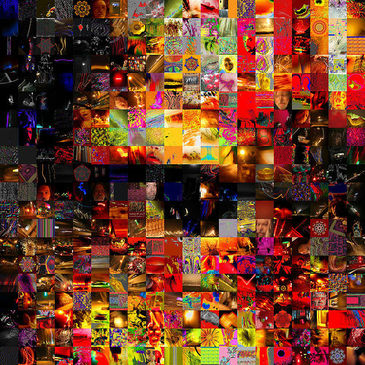
\includegraphics[width=0.3\textwidth]{eye}
    \caption{A high dimensional space (many images). }
    \end{center}
\end{figure}

We turn to Markov chain Monte Carlo (MCMC).

}



\frame{
\frametitle{Intution}

Imagine that we have a complicated function $f$ below and it's high probability regions are represented in green.

\begin{figure}
  \begin{center}
    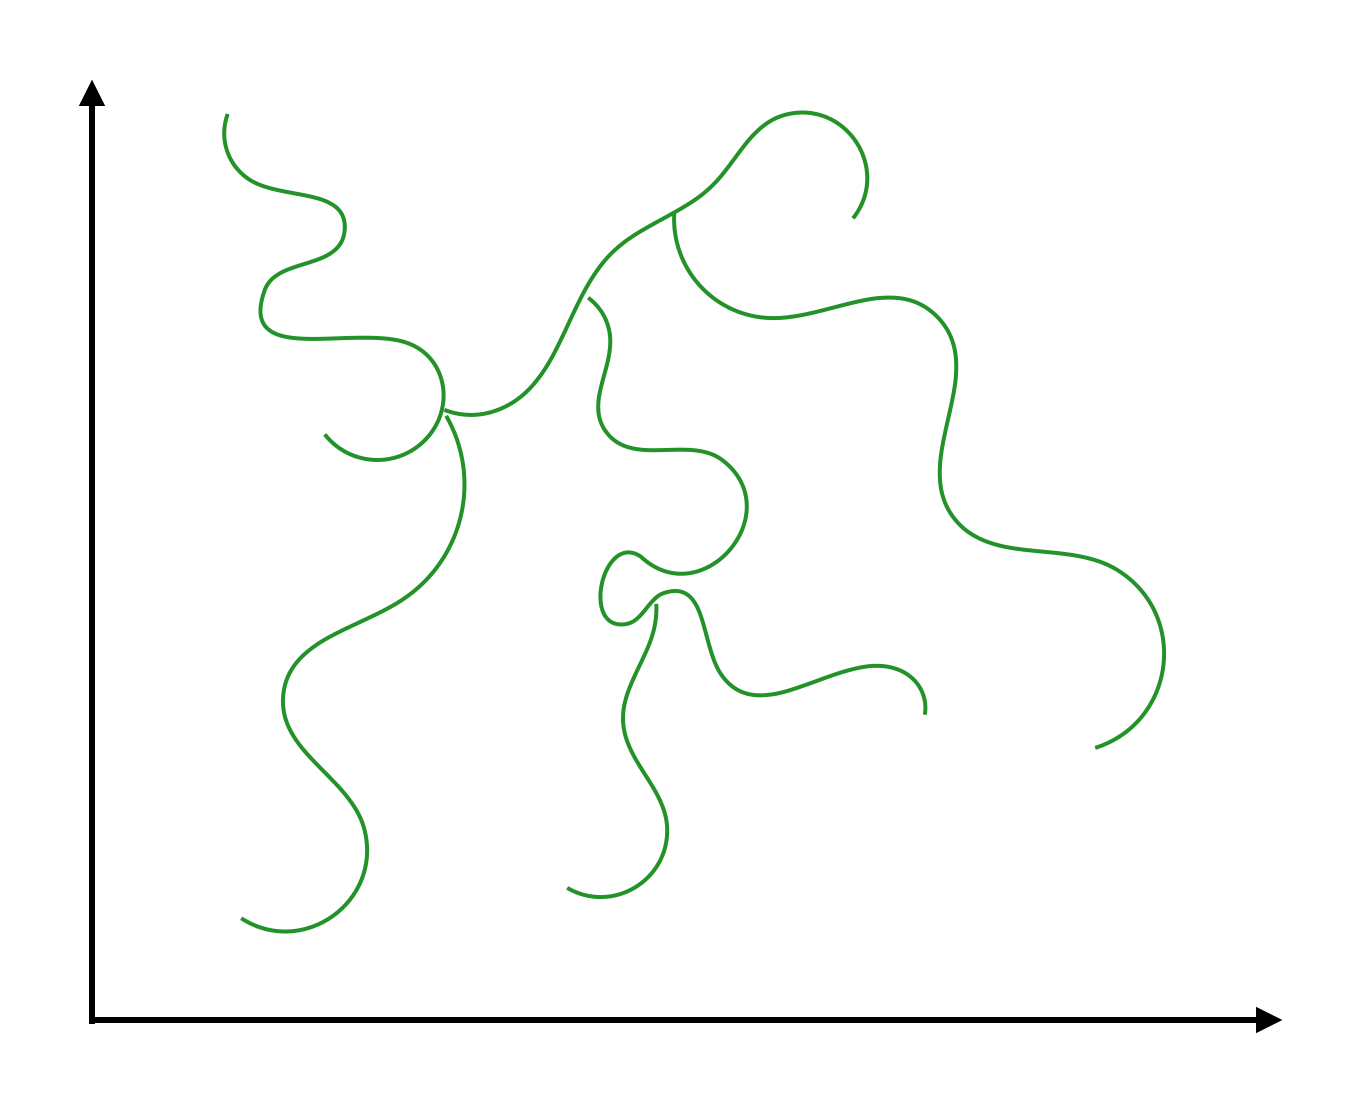
\includegraphics[width=0.7\textwidth]{markovChain}
    \caption{Example of a Markov chain}
    \end{center}
\end{figure}

}

\frame{
\frametitle{Intution}



\begin{figure}
  \begin{center}
    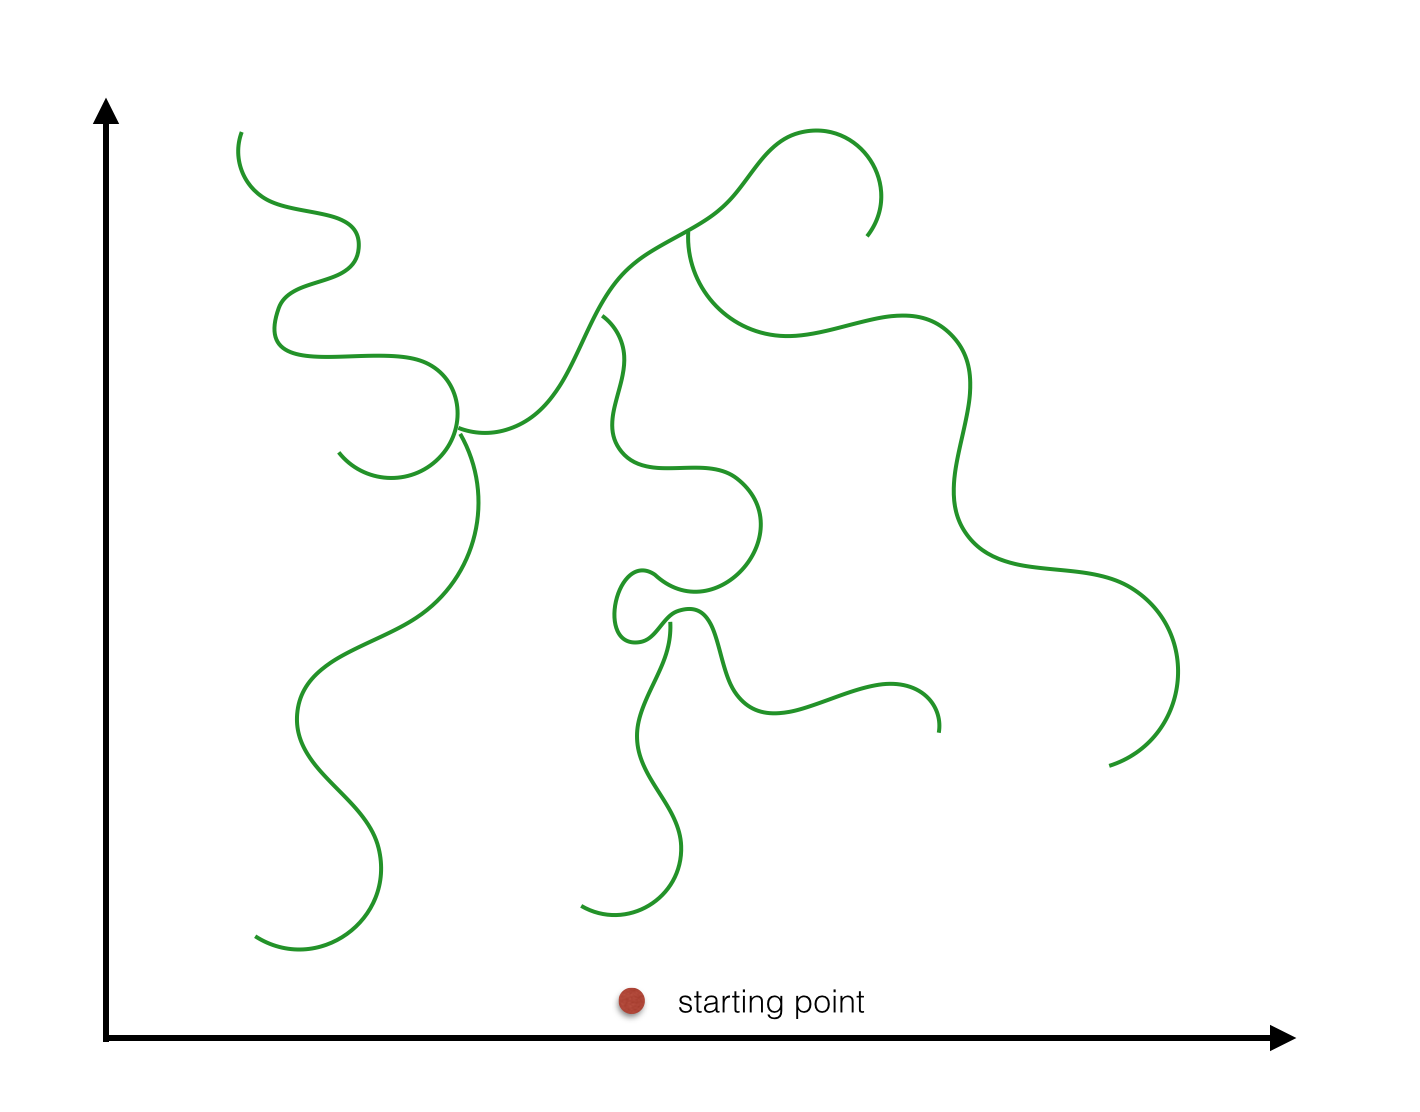
\includegraphics[width=0.7\textwidth]{markovChainPoint}
    \caption{Example of a Markov chain and red starting point}
    \end{center}
\end{figure}

}

\frame{
\frametitle{Intution}

\begin{figure}
  \begin{center}
    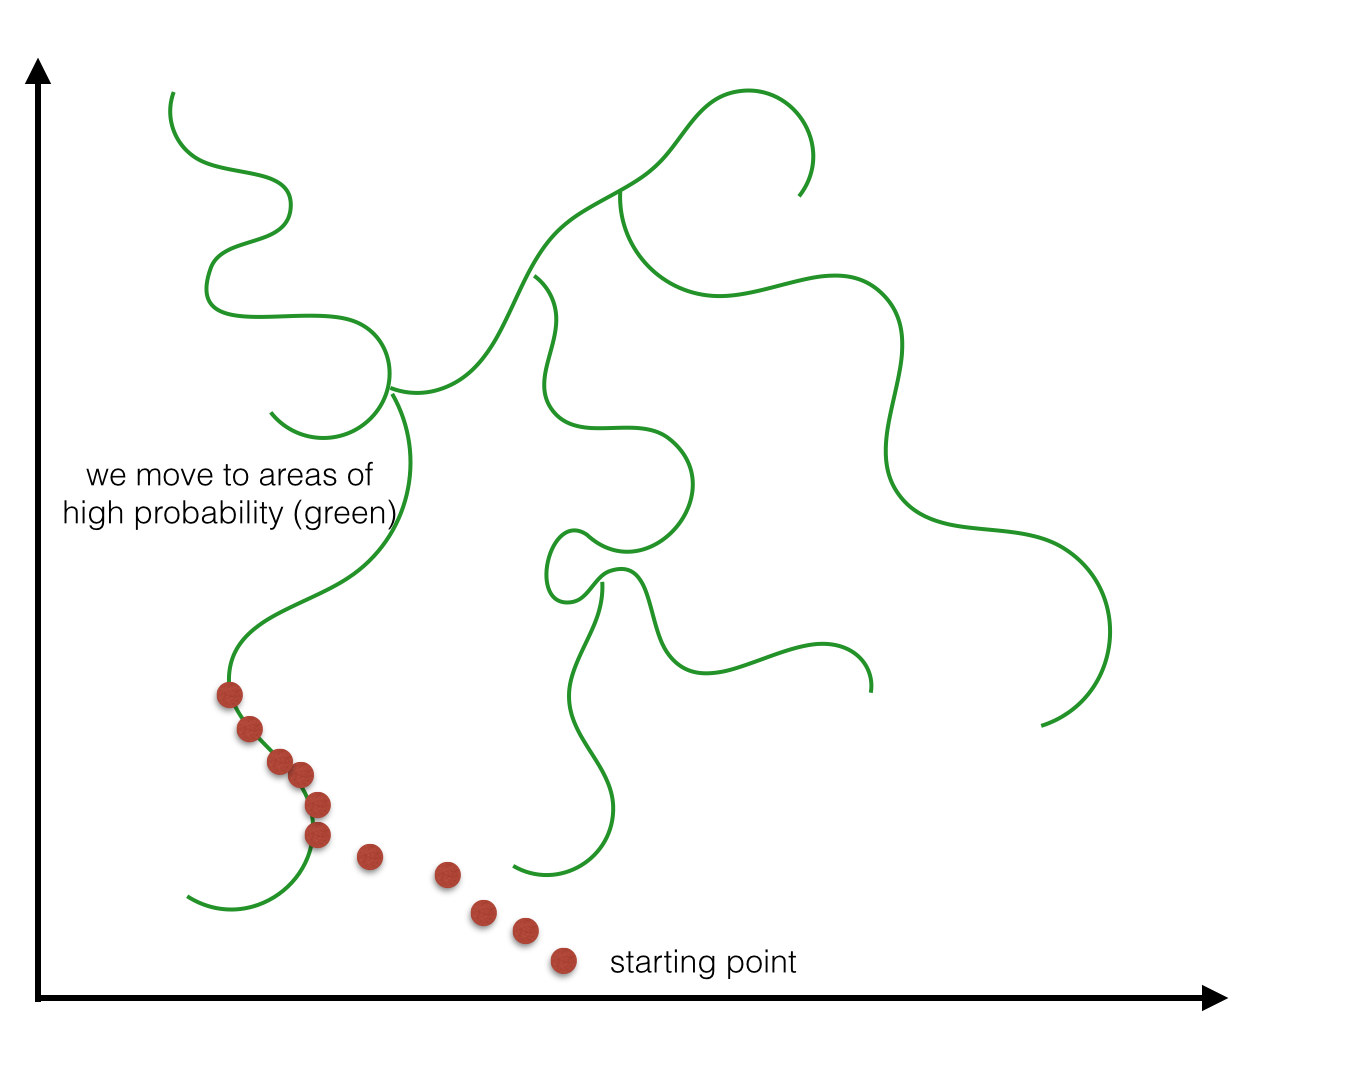
\includegraphics[width=0.7\textwidth]{markovChainMove}
    \caption{Example of a Markov chain and moving from the starting point to a high probability region.}
    \end{center}
\end{figure}

}



\frame{
\frametitle{What is Markov Chain Monte Carlo}

\begin{itemize}
\item Markov Chain -- where we go next only depends on our last state (the Markov property).
\item Monte Carlo -- just simulating data. 
\end{itemize}



}



\frame{
\frametitle{Why MCMC?}

\begin{itemize}
\item[(a)] the region of high probability tends to be ``connected''
\item That is, we can get from one point to another without going through a low-probability region, and
\item[(b)] we tend to be interested in the expectations of functions that are relatively smooth and have lots of ``symmetries''
\item  That is, one only needs to evaluate them at a small number of representative points in order to get the general picture.
\end{itemize}

}


\frame{
\frametitle{Advantages/Disadvantages of MCMC:}
Advantages:
\begin{itemize}
\item applicable even when we can't directly draw samples
\item works for complicated distributions in high-dimensional spaces, even when we don't know where the regions of high probability are
\item relatively easy to implement
\item fairly reliable
\end{itemize}

{Disadvantages:}
\begin{itemize}
\item slower than simple Monte Carlo or importance sampling (i.e., requires more samples for the same level of accuracy)
\item can be very difficult to assess accuracy and evaluate convergence, even empirically
% \item theoretical guarantees on convergence rates are difficult to obtain
\end{itemize}

}



\frame{
\frametitle{Hard Discs in a Box Example}


\begin{figure}
  \begin{center}
    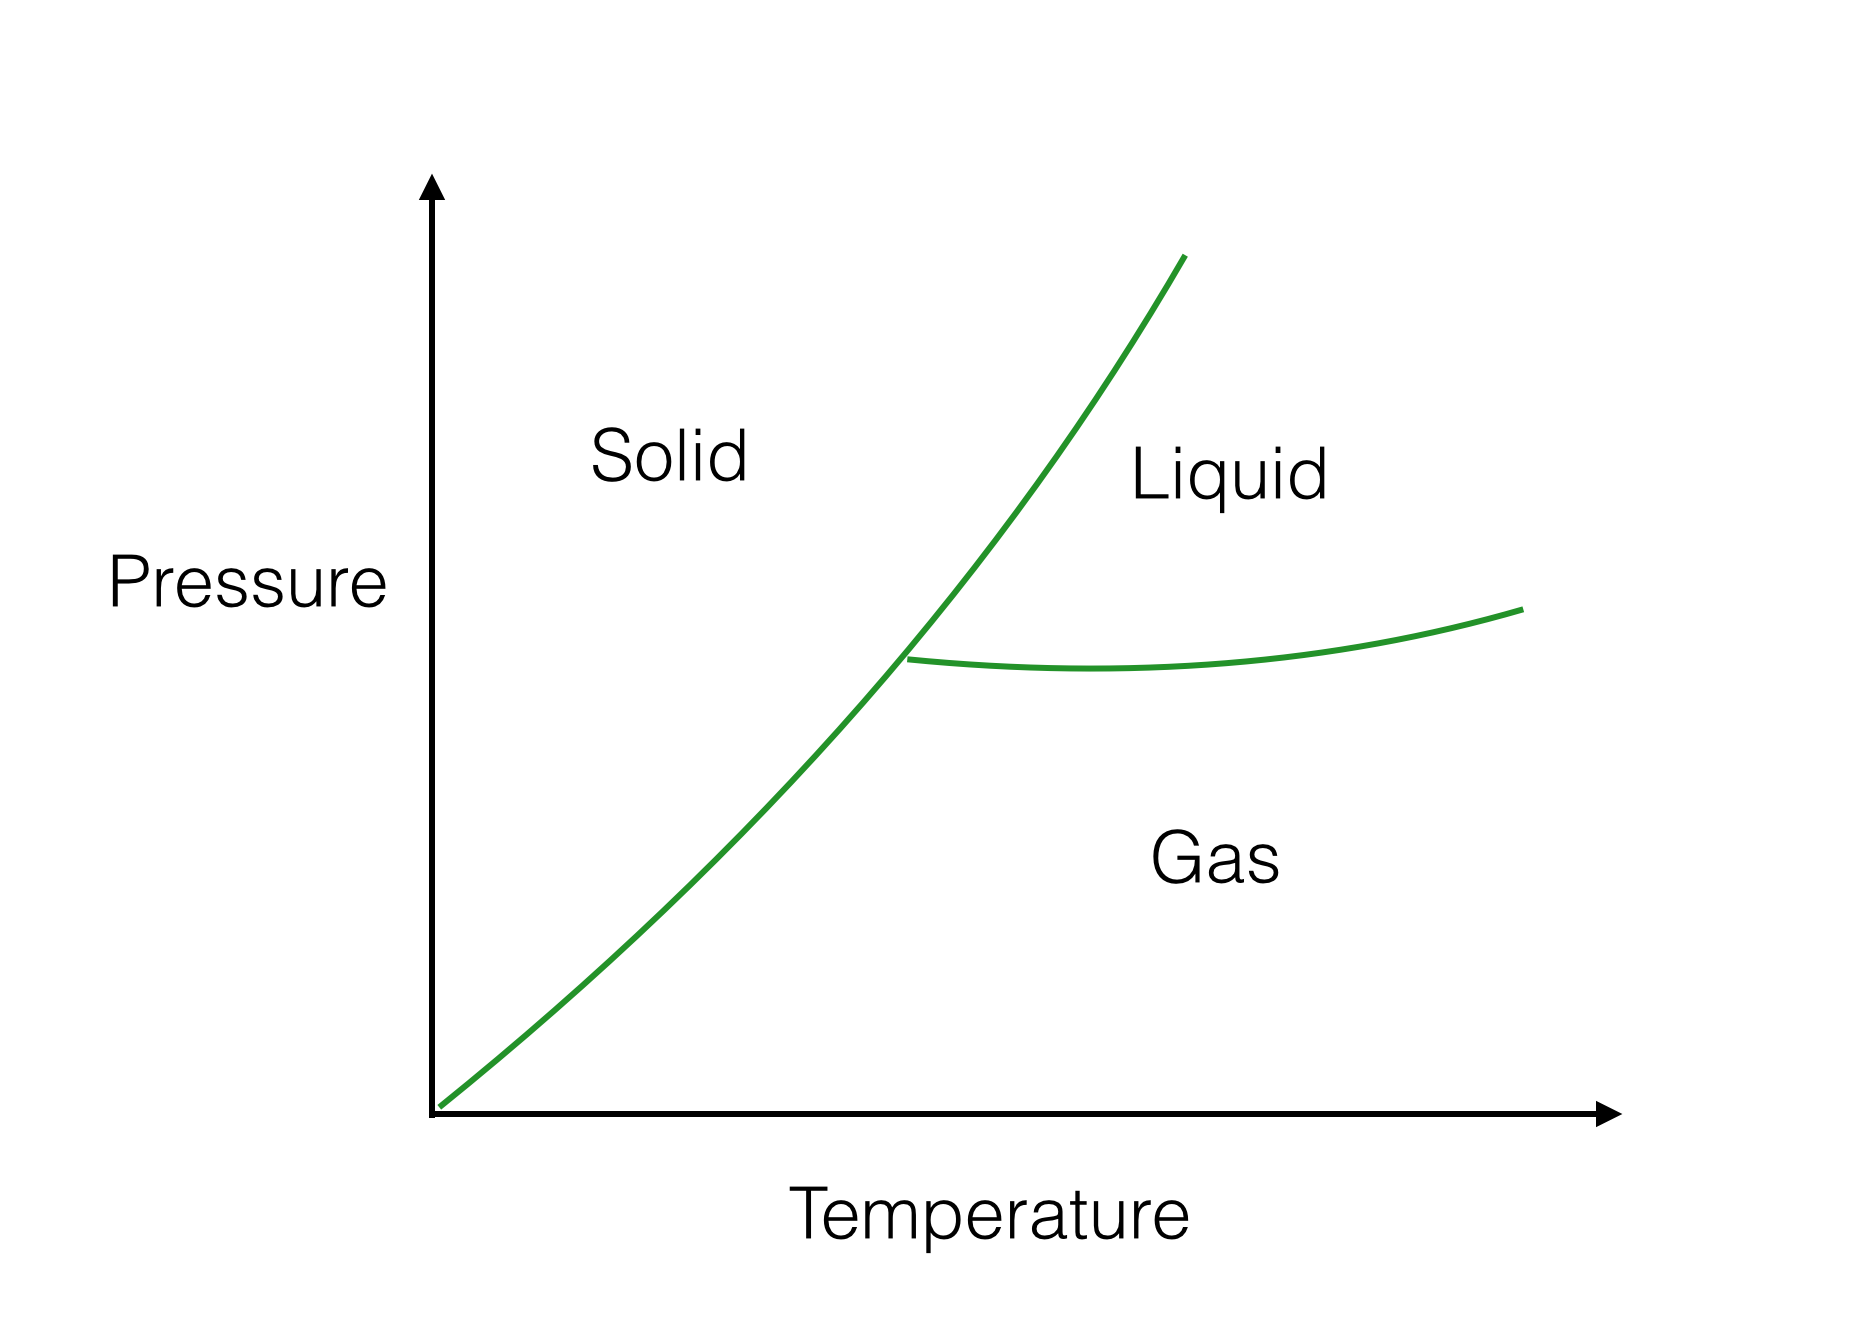
\includegraphics[width=0.8\textwidth]{phaseDiagram}
    \caption{Example of a phase diagram in chemistry.}
    \end{center}
\end{figure}

Many materials have phase diagrams that look like the picture above. 




}



\frame{
\frametitle{Hard Discs in a Box Example}
To understand this phenoma, a theoretical model was proposed:
\href{http://www.aliquote.org/pub/metropolis-et-al-1953.pdf}{Metropolis, Rosenbluth, Rosenbluth, and Teller, 1953}

\vskip 1em


\begin{figure}
  \begin{center}
    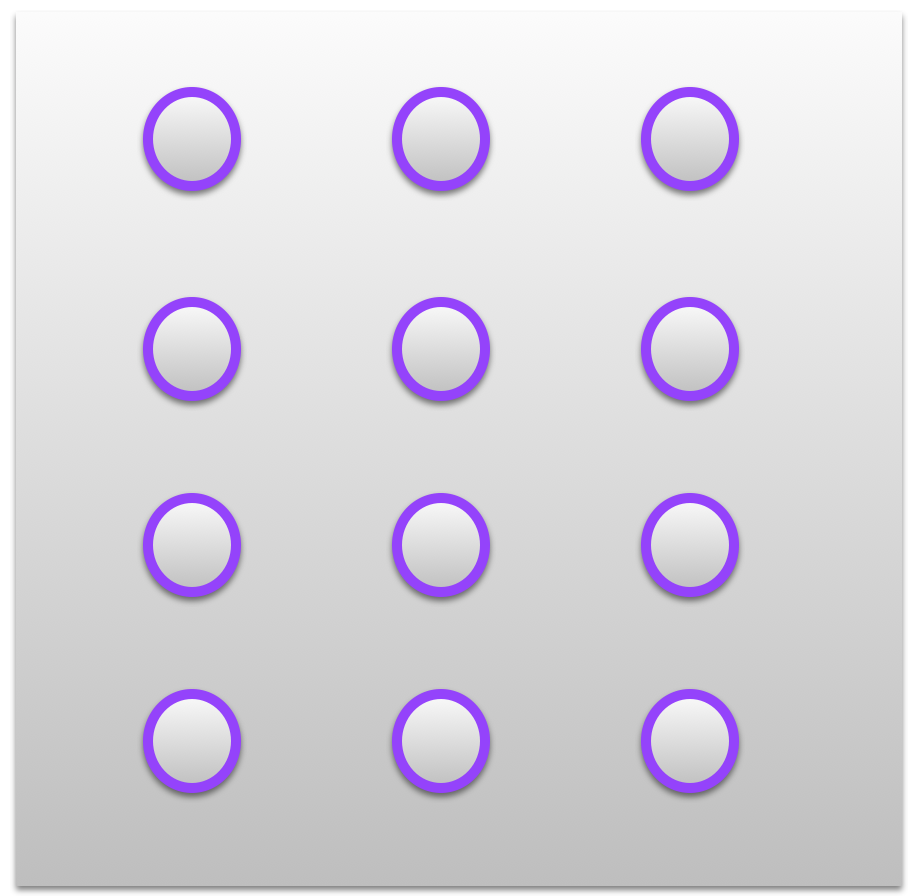
\includegraphics[width=0.4\textwidth]{hardDiscs}
    \caption{Example of $N$ molecules (hard discs) bouncing around in a box.}
    \end{center}
\end{figure}
\vskip 1em

Called hard discs because the molecules cannot overlap. 



}

\frame{
\frametitle{Hard Discs in a Box Example}
Have an $(x,y)$ coordinate for each molecule.
\vskip 1em
The total dimension of the space is $\mathbb{R}^{2N}.$

\begin{figure}
  \begin{center}
    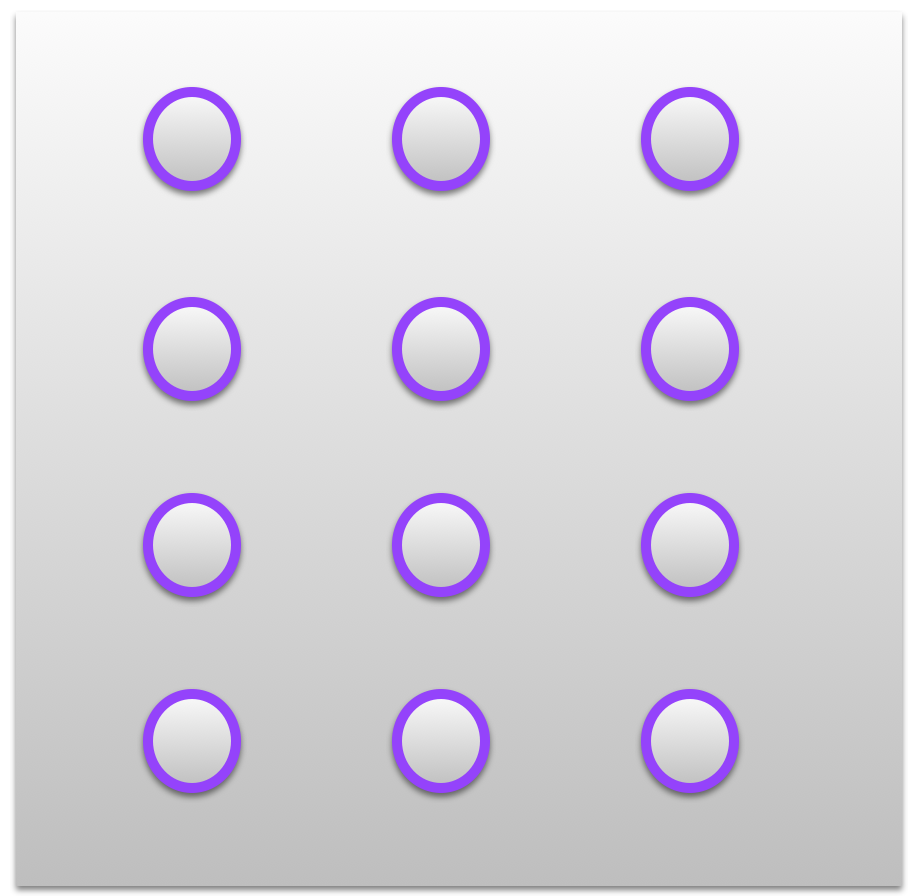
\includegraphics[width=0.4\textwidth]{hardDiscs}
    \caption{Example of $N$ molecules (hard discs) bouncing around in a box.}
    \end{center}
\end{figure}


}

\frame{
\frametitle{Hard Discs in a Box Example}
$X \sim f(x)$ (Boltzman distribution). 

\vskip 1em
Goal: compute $E_f[h(x)].$

\vskip 1em
Since $X$ is high dimensional, they proposed ``clever moves" of the molecules. 
}

%\frame{
%\frametitle{High Level Overview of Metropolis Algorithm}
%Metropolis algorithm:
%\begin{enumerate}
%\item Consider a molecule and a box around the molecule.
%\item Uniformly draw a point in the box.
%\item According to a ``rule", you accept or reject the point. 
%\item If it's accepted, you move the molecule. 
%\end{enumerate}
%Repeat. 
%
%
%
%\begin{figure}
%  \begin{center}
%    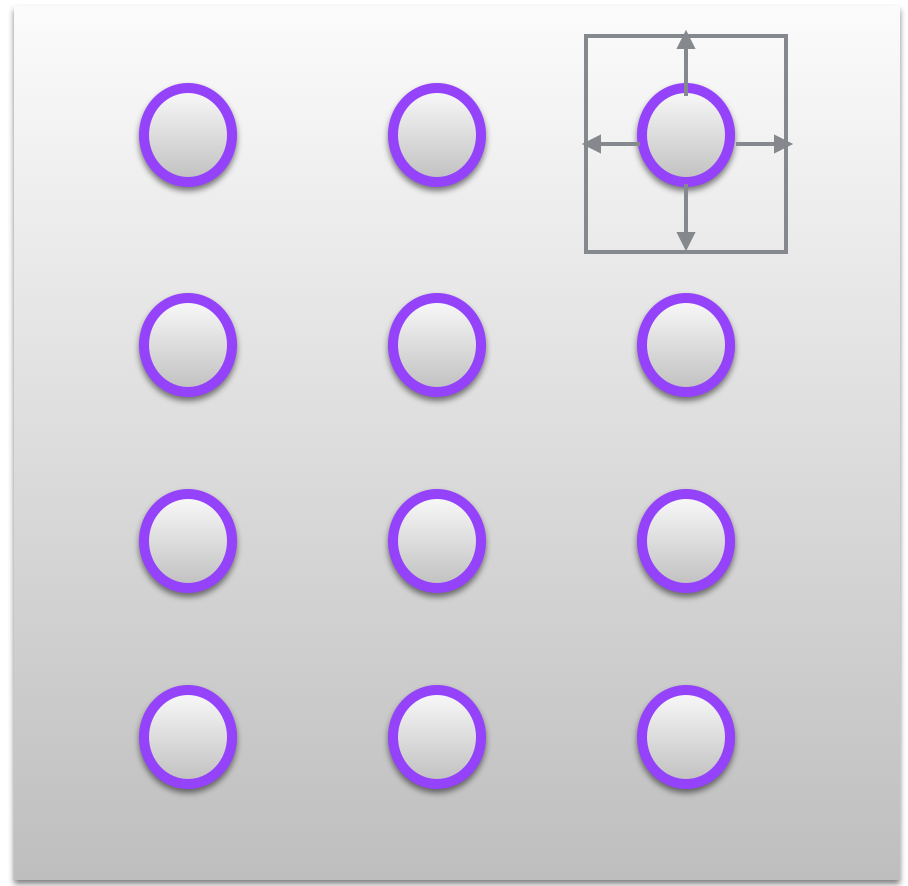
\includegraphics[width=0.4\textwidth]{hardDiscsUniform}
%    \caption{This illustrates step 1 of the algorithm.}
%    \end{center}
%\end{figure}
%
%}

\frame{
\frametitle{High Level Overview of Metropolis Algorithm}
Metropolis algorithm: For iterations $i=1,\ldots,n$, do:
\begin{enumerate}
\item Consider a molecule and a box around the molecule.
\item Uniformly draw a point in the box.
\item According to a ``rule", you accept or reject the point. 
\item If it's accepted, you move the molecule. 
\end{enumerate}
[For clarification, you could use this as pseudocode on the exam instead of writing
R code.]




}

\frame{
\frametitle{Example of one iteration of algorithm}

Consider a molecule and a box around the molecule.

\begin{figure}
  \begin{center}
    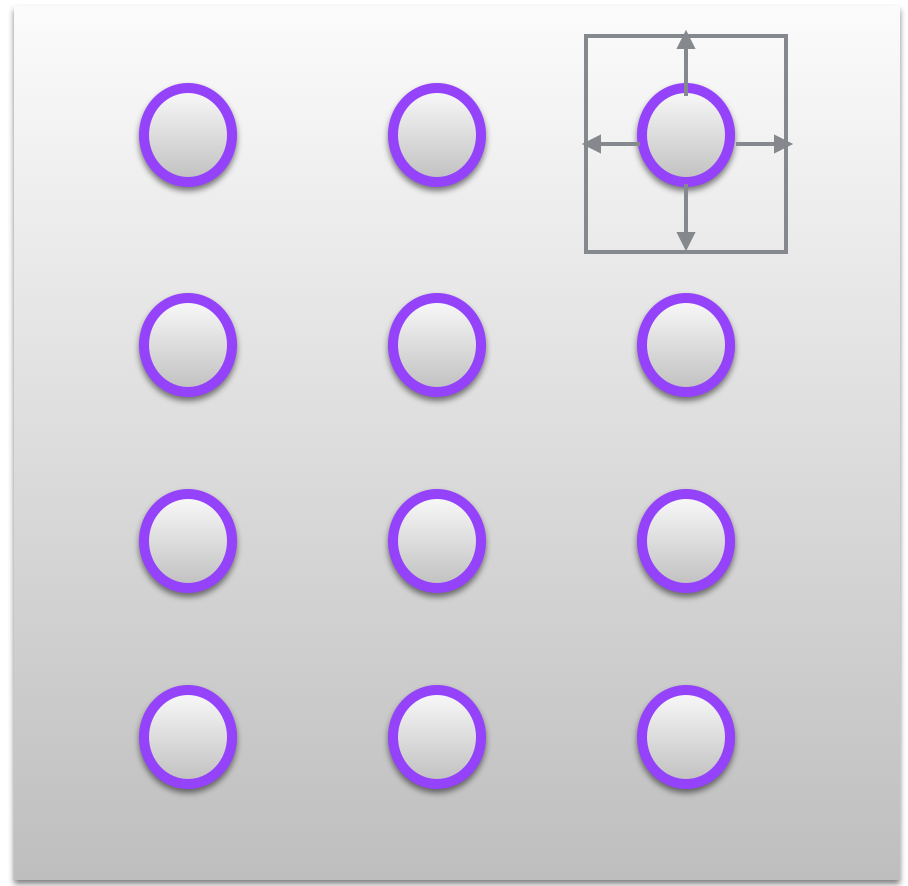
\includegraphics[width=0.4\textwidth]{hardDiscsUniform}
    \caption{This illustrates step 1 of the algorithm.}
    \end{center}
\end{figure}





}



\frame{
\frametitle{Example of one iteration of algorithm}

Uniformly draw a point in the box.

\begin{figure}
  \begin{center}
    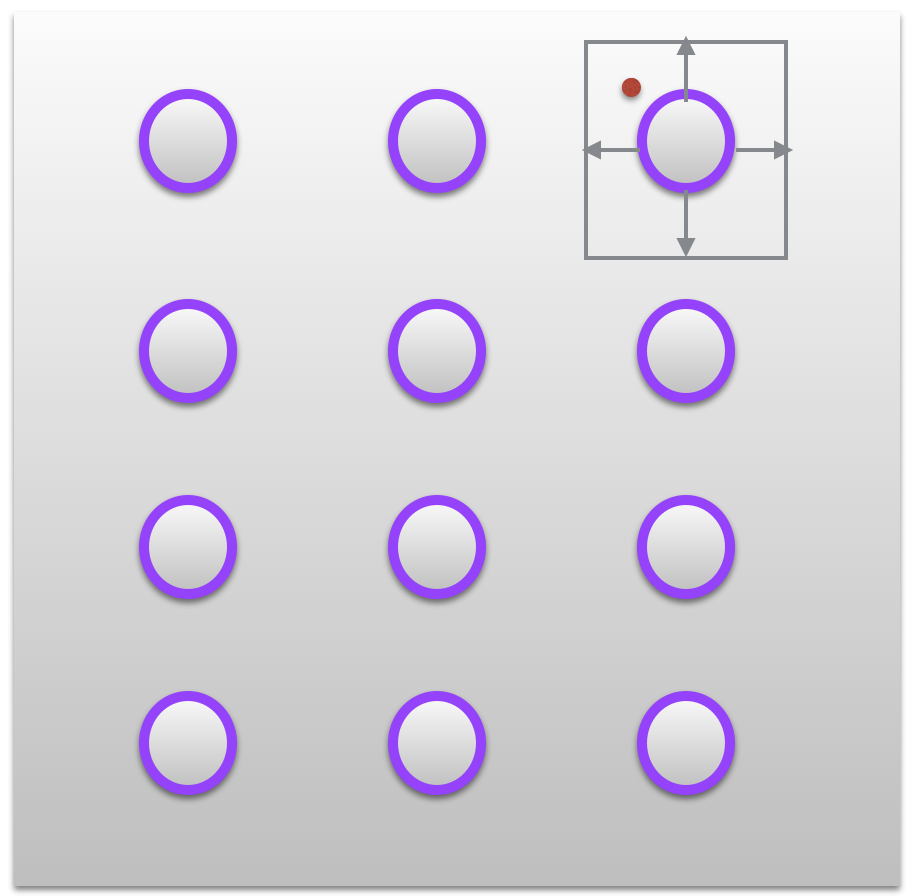
\includegraphics[width=0.4\textwidth]{hardDiscsPoint}
    \caption{This illustrates step 2 of the algorithm.}
    \end{center}
\end{figure}





}


\frame{
\frametitle{Example of one iteration of algorithm}

According to a ``rule", you accept or reject the point. 

\vskip 1em

Here, it was accepted, so we move the point. 

\begin{figure}
  \begin{center}
    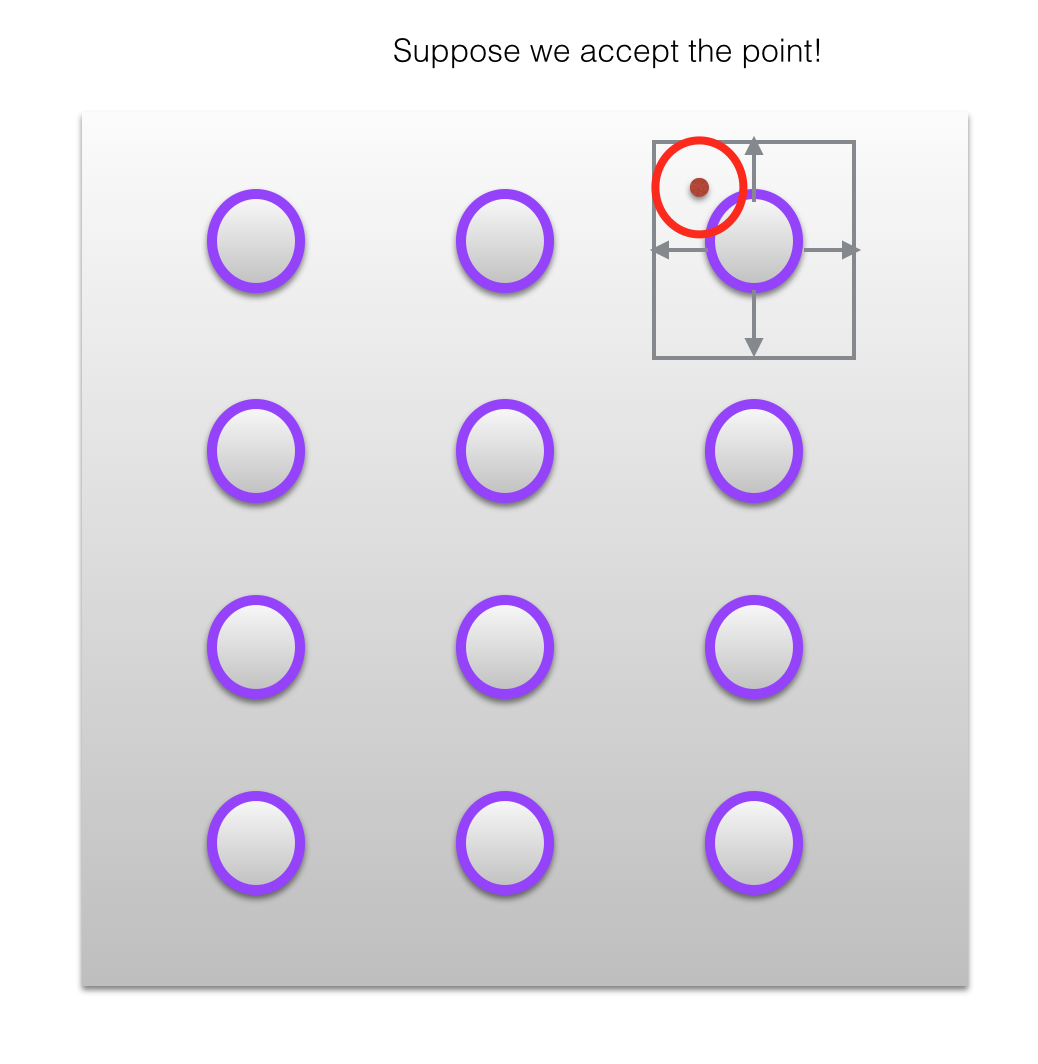
\includegraphics[width=0.4\textwidth]{hardDiscsAccept}
    \caption{This illustrates step 3 and 4 of the algorithm.}
    \end{center}
\end{figure}





}

\frame{
\frametitle{Example of one iteration of algorithm}

Here, we show one entire iteration of the algorithm.

\begin{figure}
  \begin{center}
    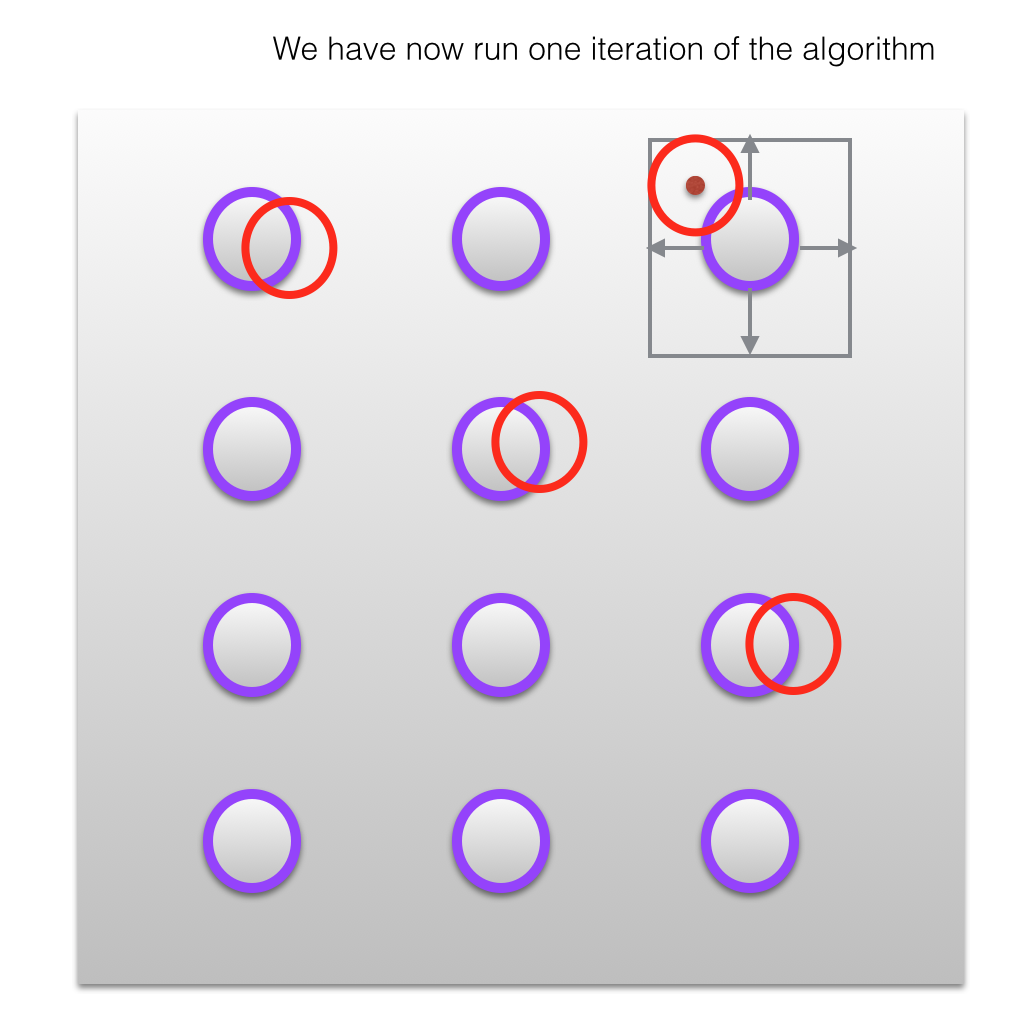
\includegraphics[width=0.4\textwidth]{hardDiscsMetropolis}
    \caption{This illustrates one iteration of the algorithm.}
    \end{center}
\end{figure}

After running many iterations $n$ (not $N$), we have an approximation for $E_f(h(X)),$ which is
$\frac{1}{n} \sum_i h(X_i).$

\vskip 1em

We will talk about the details later of why this is a ``good approximation."

}

\frame{
\frametitle{Some food for thought}
We just covered the Metropolis algorithm (1953 paper). 
\begin{itemize}
\item We did not cover the exact procedure for accepting or rejecting (to come). 
\item Are the $X_i$'s independent? 
\item Our approximation holds by \href{https://www.youtube.com/watch?v=ZjrJpkD3o1w}{The Ergodic Theorem} \\
for those that want to learn more about it.
\item The ergodic theorem says: ``if we start at a point $x_o$ and we keeping moving around in our high dimensional space, then we are guaranteed to eventually reach all points in that space with probability 1."
\end{itemize}
}

\frame{
\frametitle{Metropolis Algorithm}

Setup: Assume pmf $\pi$ on $\mathcal{X}$ (countable).

\vskip 1em

Have $f: \mathcal{X} \rightarrow \mathbb{R}.$

\vskip 1em

Goal: 
\begin{enumerate}
\item[a)] sample/approximate from $\pi$
\item[b)] approximate $E_\pi[f(x)], X\sim \pi.$
\end{enumerate}

The assumption is that $\pi$ and or $f(X)$ are complicated!
}

\frame{
\frametitle{Why things work!}
Big idea and why it works: we apply the ergodic theorem.
\vskip 1em

``If we take samples $X = (X_0,X_1,\ldots,)$ then by the ergodic theorem, they will eventually reach $\pi$, which is known as the stationary distribution (the true pmf)."


}

\frame{
\frametitle{Metropolis Algorithm}
The approach is to apply the ergodic theorem. 

%It allows two things to happens that are nice. 

\begin{enumerate}
\item If we run the Markov chain long enough, then the last state is approximately from $\pi.$
\item Under some regularly conditions, 
$$\frac{1}{n}\sum_{i=1}^n f(X_i) \stackrel{a.s}{\longrightarrow} E_\pi[f(x)].$$
\end{enumerate}



}

\frame{
\frametitle{Terminology}

\begin{enumerate}

\item Proposal matrix = stochastic matrix. 

\vskip 1em

Let $$Q = (Q_{ab}: a,b \in \mathcal{X}).$$

\vskip 1em

Note: I will use $Q_{ab} = Q(a,b)$ at times. 

\item Note: $$\pi(x) = \tilde{\pi}(x)/z, z>0.$$
What is known and unknown above?
\end{enumerate}


}

\frame{
\frametitle{Metropolis Algorithm}

\begin{itemize}
\item Choose a symmetric proposal matrix $Q.$ So, $Q_{ab} = Q_{ba}.$
\item Initialize $x_o \in X.$
\item for $i \in 1,2,\ldots,n-1$:
\begin{itemize}
\item Sample proposal $x$ from $Q(x_i, x) = p(x \mid x_i).$
\item Sample $\textcolor{red}{r}$ from Uniform$(0,1).$
\item If $$r < \frac{\tilde{\pi}(x)}{\tilde{\pi}(x_i)},$$ accept and $x_{i+1} = x.$
\item Otherwise, reject and $x_{i+1} = x_i.$
\end{itemize}
\end{itemize}
You do not need to know the general proof of this.

}

\frame{
\frametitle{Metropolis within a Bayesian setting}

Goal: We want to sample from $$p(\theta \mid y)= \frac{f(y \mid \theta) \pi(\theta)}{m(y)}.$$

\vskip 1em

Typically, we don't know $m(y).$

\vskip 1em

The notation is a bit more complicated, but the  set up is the same.

\vskip 1em 

We'll approach it a bit differently, but the idea is exactly the same. 



}

\frame{
\frametitle{Building a Metropolis sampler}
We know $\pi(\theta)$ and $f(y\mid \theta)$, so we can can draw samples from these. 

\vskip 1 em

Our notation here will be that we assume parameter values $\theta_1,\theta_2,\ldots,\theta_s$ which are drawn from $\pi(\theta).$

\vskip 1 em

We assume a new parameter value comes in that is $\theta^*.$

}

\frame{

Similar to before we assume a symmetric proposal distribution, which we call $J(\theta^* \mid \theta^{(s)}).$

\vskip 1 em




%Suppose we are interested in computing $E_\pi[g(\theta) \mid y].$ 
%We should be able to approximate this via $1/n \sum_i g(\theta^(i))$
%by the ergodic theorem. 


%How might we intuitively construct such a collection? 

%\begin{itemize}
%\item Suppose we have a working collection 
%$\{
%\theta^{(1)},\ldots, \theta^{(s)}
%\}$ and we want to add a new value $\theta^{(s+1)}.$
%\item Consider adding a value $\theta^*$ which is nearby 
%$ \theta^{(s)}.$
%\item Should we include $\theta^*$ or not?
%\item If $p(\theta^* | y) > p(\theta^{(s)} | y),$ then we want more $\theta^*$'s in the set than $\theta^{(s)}$'s.
%\item But if $p(\theta^* | y) < p(\theta^{(s)} | y),$ we shouldn't necessarily include $\theta^*.$
%\end{itemize}
%Based on the above, perhaps our decision to include $\theta^*$ or not should be based upon a comparison of $p(\theta^* | y)$ and  $p(\theta^{(s)} | y).$ We can do this by computing r:
%
%
%$$r = \dfrac{p(\theta^*|y)}{p(\theta^{(s)}|y)} = \dfrac{p(y \mid \theta^*)p(\theta^*)}
%{p(y \mid \theta^{(s)})p(\theta^{(s)})}.
%$$
%
%Having computed $r,$ what should we do next? 
%
%\begin{itemize}
%\item If $r>1$ \textcolor{blue}{(intuition)}: Since $\theta^{(s)}$ is already in our set, we should include $\theta^*$ as it has a higher probability than $\theta^{(s)}.$\\
%
% \textcolor{red}{(procedure)}:  Accept $\theta^*$ into our set and let $\theta^{(s+1)} = \theta^*.$
%\item If $r<1$
% \textcolor{blue}{(intuition)}: The relative frequency of $\theta$-values in our set equal to $\theta^*$ compared to those equal to $\theta^{(s)}$ should be 
%$$\dfrac{p(\theta^*|y)}{p(\theta^{(s)}|y)} = r. $$ This means that for every instance of 
%$\theta^{(s)},$ we should only have a fraction of an instance of a $\theta^*$ value. \\
%
% \textcolor{red}{(procedure)}:  Set $\theta^{(s+1)} $ equal to either $\theta^*$ or $\theta^{(s)} $ with probability $r$ and $1-r$ respectively. 
%\end{itemize} 


\begin{itemize}
%\item It proceeds by sampling a proposal value $\theta^*$ nearby the current value 
%$\theta^{(s)}$ using a \emph{symmetric proposal distribution} $J(\theta^* \mid \theta^{(s)}).$
\item What does symmetry mean here? 
$J(\theta_a \mid \theta_b) = J(\theta_b \mid \theta_a).$ 
\item That is, the probability of proposing $\theta^* = \theta_a$ given that $\theta^{(s)} = \theta_b$ is equal to the probability of proposing 
$\theta^* = \theta_b$ given that $\theta^{(s)} = \theta_a.$
\item Symmetric proposals include:\\
$$J(\theta^*\mid \theta^{(s)}) = \text{Uniform}(\theta^{(s)} - \delta, \theta^{(s)} + \delta)$$
and
$$J(\theta^*\mid \theta^{(s)}) = \text{Normal}(\theta^{(s)}, \delta^2).$$
\end{itemize} 

}

\frame{

The Metropolis algorithm proceeds as follows:
\begin{enumerate}
\item Sample $\theta^* \sim J(\theta \mid \theta^{(s)}).$
\item Compute the acceptance ratio (r):
$$r = \dfrac{p(\theta^*|y)}{p(\theta^{(s)}|y)} = \dfrac{p(y \mid \theta^*)p(\theta^*)}
{p(y \mid \theta^{(s)})p(\theta^{(s)})}.
$$
\item Let $$\theta^{(s+1)} =\begin{cases}
\theta^* &\mbox{with prob min(r,1)}  \\
\theta^{(s)} & \mbox{otherwise. } \end{cases} 
$$
\end{enumerate}
Remark: Step 3 can be accomplished by sampling $u \sim \text{Uniform}(0,1)$ and setting 
$\theta^{(s+1)} = \theta^*$ if $u<r$ and setting $\theta^{(s+1)} = \theta^{(s)}$  otherwise.
\vskip 1em
Exercise: Convince yourselves that step 3 is the same as the remark!



}

\frame{
\frametitle{A Toy Example of Metropolis}


Let's test out the Metropolis algorithm for the conjugate Normal-Normal model with a known variance situation. 

 
\begin{align*}
X_1,\ldots,X_n\mid \theta &\stackrel{iid}{\sim} \text{Normal}(\theta, \sigma^2)\\
\theta &\sim \text{Normal}(\mu, \tau^2).\\
\end{align*}
Recall that the posterior of $\theta$ is Normal$(\mu_n, \tau_n^2),$
where
$$\mu_n = \bar{x}\frac{n/\sigma^2}{n/\sigma^2+1/\tau^2}
+
 \mu \frac{1/\tau^2}{n/\sigma^2+1/\tau^2}$$
 and 
 $$ \tau_n^2 = \frac{1}{n/\sigma^2+1/\tau^2}.$$

}

\frame{
\frametitle{A Toy Example of Metropolis}

In this example: $\sigma^2 =1,$ $\tau^2 = 10,$ $\mu =5,$ $n = 5, $ and 
$$y = (9.37, 10.18,9.16,11.60,10.33).$$ For these data, $\mu_n = 10.03$ and 
$\tau^2_n = 0.20.$

\vskip 1em

Note: this is a toy example for illustration. 

%Suppose that for some ridiculous reason we cannot come up with the posterior distribution and instead we need the Metropolis algorithm to approximate it (please note how incredible silly this example is and it's just to illustrate the method). 

}

\frame{

We need to compute the acceptance ratio $r.$
%\vskip 1em
%Notation: $p(\theta^{*}|x)$ denotes the the posterior given a NEW data point.  $p(\theta^{(s)}|x)$ denotes the posterior from the original sample.
%
%\vskip 1em
Then

\begin{align}
r &= \dfrac{p(\theta^{*}|x)}{p(\theta^{(s)}|x)} \\
&= 
\dfrac{
p(x|\theta^{*})p(\theta^{*})
}
{
p(x|\theta^{(s)})
p(\theta^{(s)})
}\\
&=\left( \frac{\prod_i\text{dnorm}(x_i, \theta^*,\sigma)}
{\prod_i \text{dnorm}(x_i, \theta^{(s)},\sigma)}
\right)
\left( \frac{ \text{dnorm}(\theta^*, \mu, \tau)}
{ \text{dnorm}(\theta^{(s)}, \mu, \tau)}
\right)
\end{align}
}

\frame{

In many cases, computing the ratio $r$ directly can be numerically unstable, however, this can be modified by taking $\log r.$ 

This results in 
\begin{align*}
&\log r =\sum_i\left[
\log  \text{dnorm}(x_i, \theta^*,\sigma) - 
\log  \text{dnorm}(x_i, \theta^{(s)},\sigma)
\right] \\
&\qquad+
\sum_i\left[
\log  \text{dnorm}(\theta^*, \mu, \tau) - 
\log  \text{dnorm}(\theta^{(s)}, \mu, \tau)
\right].
\end{align*}
Then a proposal is accepted if $\log u < \log r,$ where $u$ is sample from the Uniform(0,1).

}

\frame{


We generate 10,000 iterations of the Metropolis algorithm starting at 
$\theta^{(0)} = 0$ and using a normal proposal distribution, where
$$\theta^{(s+1)} \sim \text{Normal}(\theta^{(s)},2).$$

 Figure~\ref{met_norm} shows a trace plot for this run as well as a histogram for the Metropolis algorithm compared with a draw from the true normal density. 
 }
 
 \frame{
 
% From the trace plot, although the value of $\theta$ does not start near the posterior mean of 10.03, it quickly arrives there after just a few iterations. The second plot shows that the empirical distribution of the simulated values is very close to the true posterior distribution. 

\begin{figure}[htbp]
\begin{center}
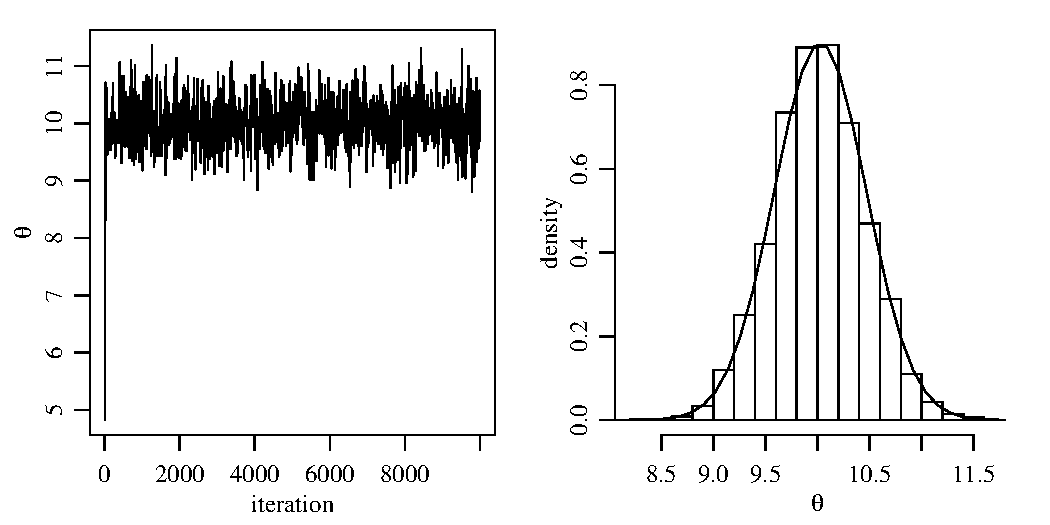
\includegraphics[scale=0.5]{metropolis_normal.pdf}
\caption{Left: trace plot of the Metropolis sampler. Right: Histogram versus true normal density for 10,000 iterations.}
\label{met_norm}
\end{center}
\end{figure}
}

\begin{frame}[fragile]
\begin{verbatim}
# setting values 
set.seed(1)
s2<-1 
t2<-10 
mu<-5; 
n<-5

# rounding the rnorm to 2 decimal places
y<-round(rnorm(n,10,1),2)
# mean of the normal posterior
mu.n<-( mean(y)*n/s2 + mu/t2 )/( n/s2+1/t2) 
# variance of the normal posterior 
t2.n<-1/(n/s2+1/t2)
# defining the data
y<-c(9.37, 10.18, 9.16, 11.60, 10.33)
\end{verbatim}
\end{frame}

\begin{frame}[fragile]
\begin{verbatim}

####metropolis part####
##S = total num of simulations
theta<-0 ; delta<-2 ; S<-10000 ; THETA<-NULL ; set.seed(1)

for(s in 1:S){
## simulating our proposal
  #the new value of theta
  theta.star<-rnorm(1,theta,sqrt(delta))

##taking the log of the ratio r
  log.r<-( sum(dnorm(y,theta.star,sqrt(s2),log=TRUE)) 
              + dnorm(theta.star,mu,sqrt(t2),log=TRUE) )  
        - ( sum(dnorm(y,theta,sqrt(s2),log=TRUE)) 
             +  dnorm(theta,mu,sqrt(t2),log=TRUE) ) 

  if(log(runif(1))<log.r) { theta<-theta.star }
##updating THETA 
  THETA<-c(THETA,theta)
}
\end{verbatim}


\end{frame}

\begin{frame}[fragile]
\begin{verbatim}

##two plots: trace of theta and 
comparing the empirical distribution
##of simulated values to the true posterior

par(mar=c(3,3,1,1),mgp=c(1.75,.75,0))
par(mfrow=c(1,2))

# creating a sequence
skeep<-seq(10,S,by=10)
# making a trace place
plot(skeep,THETA[skeep],type="l",
xlab="iteration",ylab=expression(theta))

# making a histogram
hist(THETA[-(1:50)],prob=TRUE,main="",
xlab=expression(theta),ylab="density")
th<-seq(min(THETA),max(THETA),length=100)
lines(th,dnorm(th,mu.n,sqrt(t2.n)) )
\end{verbatim}


\end{frame}

\frame{
\frametitle{Questions you should be able to answer!}
\begin{itemize}
\item What is the goal of Metropolis?
\item What is known and unknown? 
\item What are good proposals? 
\item What does the ergodic theorem say in words?
\item Are good proposals always easy to choose?
\item When would we use Metropolis over Importance sampling
and Rejection sampling? 
\item What is a simple diagnostic of a Markov chain?
\item Are we guaranteed convergence of the Markov chain?
\end{itemize}



}



\end{document}